\documentclass[journal=jacsat,manuscript=article,layout=twocolumn]{achemso}
%   \usepackage[version=3]{mhchem} % Formula subscripts using \ce{}
\usepackage[T1]{fontenc}       % Use modern font encodings
% \usepackage[active]{preview}
%EXTRA PACKAGES%
% \usepackage{multicol}
\usepackage{xcolor}
\usepackage{textcomp}
\usepackage{geometry}
\usepackage[normalem]{ulem}
\usepackage{amsmath}
\usepackage{amssymb}
% \usepackage{showkeys}
%%%%%%%%%%%%%%%%%%%%%%%%%%%%%%%%%%%%%%%%%%%%%%%%%%%%%%%%%%%%%%%%%%%%%
%% Place any additional macros here.  Please use \newcommand* where
%% possible, and avoid layout-changing macros (which are not used
%% when typesetting).
%%%%%%%%%%%%%%%%%%%%%%%%%%%%%%%%%%%%%%%%%%%%%%%%%%%%%%%%%%%%%%%%%%%%%
\newcommand*{\ga}{\alpha}
\newcommand*{\gb}{\beta}
\newcommand*{\gam}{\gamma}
\newcommand*{\gd}{\delta}
\newcommand*{\eps}{\epsilon}
\newcommand*{\veps}{\varepsilon}
\newcommand*{\gz}{\zeta}
\newcommand*{\gt}{\theta}
\newcommand*{\gi}{\iota}
\newcommand*{\gk}{\kappa}
\newcommand*{\gl}{\lambda}
\newcommand*{\gs}{\sigma}
\newcommand*{\go}{\omega}
\newcommand*{\Gam}{\Gamma}
\newcommand*{\gD}{\Delta}
\newcommand*{\gT}{\Theta}
\newcommand*{\gL}{\Lambda}
\newcommand*{\gS}{\Sigma}
\newcommand*{\gO}{\Omega}
\newcommand*{\pt}[1]{\left( #1\right)}
\newcommand*{\pq}[1]{\left[ #1 \right]}
\newcommand*{\pg}[1]{\left\{ #1\right\}}
\newcommand*{\figref}[1]{\figurename~\ref{#1}}
\newcommand*{\red}[1]{\textcolor{red}{#1}}
\newcommand*{\blue}[1]{\textcolor{blue}{#1}}
\newcommand*{\gray}[1]{\textcolor{gray}{#1}}
% \renewcommand{\baselinestretch}


%%%%%%%%%%%%%%%%%%%%%%%%%%%%%%%%%%%%%%%%%%%%%%%%%%%%%%%%%%%%%%%%%%%%%
%% Meta-data block
%% ---------------
%% Each author should be given as a separate \author command.
%%
%% Corresponding authors should have an e-mail given after the author
%% name as an \email command. Phone and fax numbers can be given
%% using \phone and \fax, respectively; this information is optional.
%%
%% The affiliation of authors is given after the authors; each
%% \affiliation command applies to all preceding authors not already
%% assigned an affiliation.
%%
%% The affiliation takes an option argument for the short name.  This
%% will typically be something like "University of Somewhere".
%%
%% The \altaffiliation macro should be used for new address, etc.
%% On the other hand, \alsoaffiliation is used on a per author basis
%% when authors are associated with multiple institutions.
%%%%%%%%%%%%%%%%%%%%%%%%%%%%%%%%%%%%%%%%%%%%%%%%%%%%%%%%%%%%%%%%%%%%%
\author{Elizaveta Guseva}
\email{elizaveta.guseva@stonybrook.edu}
\affiliation[Stony Brook University]
{Laufer Center for Physical and Quantitative Biology, Stony Brook University, Stony Brook, NY, 
(United States)}
% \altaffiliation{A shared footnote}
\author{Ronald N Zuckermann}
\affiliation{Lawrence Berkeley National Laboratory (LBNL), Berkeley, CA (United States)}
\author{Ken A Dill}
\email{dill@laufercenter.org}
\phone{+1631 632 5400}
\fax{+1631 632 5405}
\affiliation[Stony Brook University]
{Laufer Center for Physical and Quantitative Biology, Stony Brook University, Stony Brook, NY, 
(United States)}


%%%%%%%%%%%%%%%%%%%%%%%%%%%%%%%%%%%%%%%%%%%%%%%%%%%%%%%%%%%%%%%%%%%%%
%% The document title should be given as usual. Some journals require
%% a running title from the author: this should be supplied as an
%% optional argument to \title.
%%%%%%%%%%%%%%%%%%%%%%%%%%%%%%%%%%%%%%%%%%%%%%%%%%%%%%%%%%%%%%%%%%%%%
\title[]{A mechanism for how prebiotic polymers may have become informational}

%%%%%%%%%%%%%%%%%%%%%%%%%%%%%%%%%%%%%%%%%%%%%%%%%%%%%%%%%%%%%%%%%%%%%
%% Some journals require a list of abbreviations or keywords to be
%% supplied. These should be set up here, and will be printed after
%% the title and author information, if needed.
%%%%%%%%%%%%%%%%%%%%%%%%%%%%%%%%%%%%%%%%%%%%%%%%%%%%%%%%%%%%%%%%%%%%%
\abbreviations{IR,NMR,UV}
\keywords{American Chemical Society, \LaTeX}

%%%%%%%%%%%%%%%%%%%%%%%%%%%%%%%%%%%%%%%%%%%%%%%%%%%%%%%%%%%%%%%%%%%%%
%% The manuscript does not need to include \maketitle, which is
%% executed automatically.
%%%%%%%%%%%%%%%%%%%%%%%%%%%%%%%%%%%%%%%%%%%%%%%%%%%%%%%%%%%%%%%%%%%%%



\begin{document}
\abstract{\footnotesize We are interested in three puzzles of how prebiotic chemistry might have 
led towards biology.  (1) Most current prebiotic chain syntheses produce only short chains, yet 
biology is thought to require longer chains.  (2) How might random sequences have selectively 
become informational?  (3) The Chemistry-to-Biology transition is thought to require 
\emph{autocatalytic sets}.  What is a plausible molecular structural basis for such sets?  Our 
hypothesis is that non-negligible fractions of random short polymers of hydrophobic ($H$) and polar 
($P$) monomers, such as constitute present-day proteins, \red{which} can collapse into relatively 
compact 
structures with exposed hydrophobic surfaces \sout{that} can act as primitive catalysts for the 
elongation 
of other such HP polymers.  Using the HP lattice model, which can explore sequence-space properties 
without bias, we find that \sout{such processes are} \red{HP-based interactions(??) indeed result 
in } autocatalytic \red{ dynamics and} lead from short chains to longer ones, 
and are sequence selective.  \red{This mechanism may be} We believe this mechanism is relevant to 
the early origins of life.}

%%%MAIN TEXT%%%%

\section{Introduction} 

 How might prebiotic polymerization processes have produced long chains of protein-like or 
 nucleic-acid-like molecules~\cite{Joyce1987,Abel2005}?  Our aim here is to identify a particular 
physical process that could have operated during the early origins of life that was 
autocatalytic; that could have produced chains that are longer than are currently observed in 
model 
prebiotic experiments; and that could have led to selective amplification of populations of 
particular sequences (on the road to biology) from underlying processes that are otherwise random 
chemical polymerizations.  
 
 The main question we ask here is how the Chemistry-To-Biology (CTB) transition might have happened 
to initiate subsequent stages of the earliest life.  Biological processes are non-equilibria that 
are both self-sustaining and self-supporting.  Our question here is not about which monomers or 
polymers were the first, or on what synthesis conditions were plausibly prebiotic.  Rather, we seek 
a physical principle of polymerization that might have spontaneously created sufficiently long 
chains, that might have led from random to informational chains, from short to long chains, and for 
a structural principle of autocatalytic sets that could be 
self-sustaining.  Here is a short summary of prior work.
 
 \section{The Autocatalysis Puzzle}
 
 Early on, it was recognized by Eigen, Kaufmann, Dyson, Prigogine and others that the CTB 
transition requires autocatalysis, \emph{i.e.} some form of positive feedback or bootstrapping 
among molecules in some 
way~\cite{eigen1971selforganization,Eigen1977,Eigen1978,Dyson1985,Prigogine1989,Kauffman1986}.  
These works postulated that autocatalysis was a necessary step for sustaining stable biochemical 
networks.  
 
 Subsequent work has been of both abstract theoretical models and experiments.  First, we review 
the theory.  There have been studies of a class of theoretical models called GARD (Graded 
Autocatalysis Replication Domain)~\cite{segre1998graded,Segre2000,Markovitch2012}, which showed 
that hypothetical autocatalytic chemico-kinetic networks should lead to self-replication, and the 
growth of concentrations of certain chemical species, which they call compositional bias.  This 
class of models focuses on mixtures of small molecules, and thus is a class of `metabolism-first' 
scenarious. While being a very interesting scenario, it does not address the question of the 
lengths and sequences of biological polymers.

Wu and Higgs~\cite{Wu2009} have developed a model of RNA chain-length autocatalysis.  They envision 
that some chains have the capability to act as polymerase ribozymes.  If so, chain length can grow 
in an autocatalytic way.  A variant of that theoretical model assumes a mechanism of 
template-assisted ligation and random breakage~\cite{Tkachenko2014}.  These authors too predict an 
autocatalytic phase transition, whereby certain conditions cause the system to produce longer 
chains and become self-sustaining.  These are abstract models insofar as they do not postulate 
molecular structures that might explain the autocatalytic step.  Nor do they address the 
heteropolymeric or informational aspects of the chains. 
Another class of abstract model does 
consider a system of random heteropolymeric sequences constructed from an alphabet of different 
monomer types~\cite{nowak2008prevolutionary,Ohtsuki2009,Chen2012,Derr2012}.  
In these models, it is 
assumed that polymers serve as their own templates.  In this case, the autopoietic mechanism is 
that a certain sequence has an ability to accelerate the growth of its own precursors, either by 
means of catalysis or replication. It was shown that for such systems replication is a more 
favorable mechanism: while in the both cases ratio of long sequences goes up, in the case 
of autocatalysis one has to increase catalysis rate exponentially in order to get exponential 
growth of, longer chains; in the same time replication also increased diversity of the population 
and compensated for possible chemical bias. These studies heavily rely on ability of chemical 
molecules to recognize ``self''. Yet in fact self-recognition a difficult question in chemistry of 
the origin of life and thus application of the studies are limited to the post-informational world.

\red{Another theoretical model\cite{Walker2012} concerned with heteropolymers studies 
informational polymers which can both go through sequence-independent template-directed replication 
and spontaneous polymerization. They study shows that such systems not only produces functional 
sequences from the pool of none-functional ones, but also effectively explores sequence space and 
keeps sequence diversity high. This agrees with Derr et al.\cite{Derr2012} findings that 
template-directed replication enhances diversity; and again, both are models of the 
post-informational world.}
 
 In addition, there have been many experimental studies.  There has been work to create artificial 
autocatalytic sets in the laboratory~\cite{VonKiedrowski1986,Lincoln2009,Vaidya2012}. Such systems 
are designed so that a pair of molecules catalyze each other, giving autocatalysis and exponential 
growth.  For example, mixtures of RNA fragments are shown to self-assemble spontaneously into 
self-replicating ribozymes that can form catalytic networks that can compete with others.  One 
limitation, however, in applying such studies to prebiotic origins is that these are fragments 
taken from existing ribozymes, so they don't address the question of the origins from more 
primitive and random beginnings.
 
  Here, we describe a theoretical model.  It differs from others in: (1) addressing the three 
questions together: chain-elongations, information growth, and autocatalysis, and (2) in giving a 
specific mechanism and structural basis for the autocatalytic process, to predict what molecules 
might be autocatalytic, with rough estimates for the rate enhancements.
 
 \section{The `Flory Problem': polymerization processes produce mostly short chains}
 \label{sec:flory} 

A key puzzle in biopolymer origins is how to produce sufficiently long chains?  Many experiments 
show that either amino acids or nucleotides can polymerize into short-chain molecules under 
prebiotic conditions without the presence of 
enzymes~\cite{Shock1992,Martin1998,PAECHT-HOROWITZ1970,Leman2004a,Orgel2004}.  It is also known 
that 
the yields of such short-chain oligomers can be increased under prebiotically plausible conditions 
by such processes as adsorption to clays~\cite{Rao1980,Lambert2008} or 
minerals~\cite{Bernal1949,Ferris1996}, by evaporation of tidal pools~\cite{Nelson2001}, by 
concentration in ice through eutectic melts~\cite{Kanavarioti2001} or freezing~\cite{Bada2004} or 
temperature cycles. 

It remains a puzzle, however, to understand how prebiotic processes could have overcome what 
we call the ``Flory Problem'' -- the production of long-chain polymers.  It is generally assumed 
that the minimum chain lengths of proteins or nucleic acids that are needed to make the complex 
structures essential for biological function is estimated to be around 30-60 monomers 
long~\cite{Szostak1993}.  Yet, since the earliest work of Flory and others, which elucidated basic 
mechanisms of chain polymerizations, it has been clear that chain syntheses are stochastic, 
whereby 
the concentrations of longer chains are exponentially smaller than of shorter chains. 

Correspondingly, experimental studies which are intended to find out possible ways of prebiotic 
polymerizations of amino acids and nucleotides lead predominantly to short chains. Leman et al. 
showed that carbonyl sulfide (COS), a simple volcanic gas, brings about the formation of 
oligo-peptides from amino acids under mild conditions in aqueous solution in minutes to hours. But
the products are mainly dimers and trimers~\cite{Leman2004a}.  In another study, using various 
mineral 
catalysts such as calcium montmorillonite, hectorite, silica or alumina, mixtures of Gly and 
Gly$_2$ 
grow to about 6-mers after 14 days~\cite{Rode1997,Rode1999}.  Or, by freezing samples of 
phosphoimidazolide-activated uridine in the presence of metal ions in dilute solutions, 
Kanavarioti 
found polymers of oligouridylates up to 11 bases long, with an average length of 4 
\cite{Kanavarioti2001}.  And, starting from decanucleotides [$^{32}$P]dA(pdA)$_8$pA adsorbed on 
Na$^+$-montmorillonite, Ferris et al. observed chains averaging lengths 20-40 after 14 days at 
25\textcelsius\ \cite{Ferris1996}.  It is not yet understood how prebiotic polymerizations could 
lead to the types of long protein or nucleic-acid chains that are found in present-day cells.

\red{A recent study~\cite{Forsythe2015} developed a prebiotically plausible mechanism of peptide 
polymerization which produces oligomers with a combination of ester and amide
bonds up to length 14 contain up to 7 amide linkages. Bond formation in this case was aided by 
likely cohabitants of early Earth amino acids $\ga$-hydroxy acids. }

The standard processes of chain polymerization lead to the the Flory or 
Flory-Schulz distribution of the concentrations of chains of different chain 
lengths~\cite{Flory1953}. 
\begin{equation}
 f(a)=a^2l(1-a)^{l-1},\label{eq:flory}
\end{equation} 
where $l$ is the chain length and $a$ is the probability of chain termination, 
which is a measure of the average chain length: $\langle l \rangle = a(2- a)$.
Figure \ref{fig:flory} shows the central prediction of Flory theory, that 
longer chains are exponentially less populated than shorter chains.  For example (see the magenta 
line 
in Fig~\ref{fig:flory}):
\begin{equation}  
\frac{\pq{10~\mathrm{mers}}}{\pq{1~\mathrm{mers}}}\propto10^{-4},\qquad\frac{\pq{20~\mathrm{mers}}}
{
\pq{1~\mathrm{mers}}}\propto10^{-9}
\end{equation} 
Thus, for a synthetic process that starts with micro-molar concentrations of monomers, the 
average chain length would be $\langle l \rangle = 2$ and 40-mers would have 
negligible concentrations of $\propto 10^{-19} $ mol/L. 
\begin{figure}[h!]
  \centering
  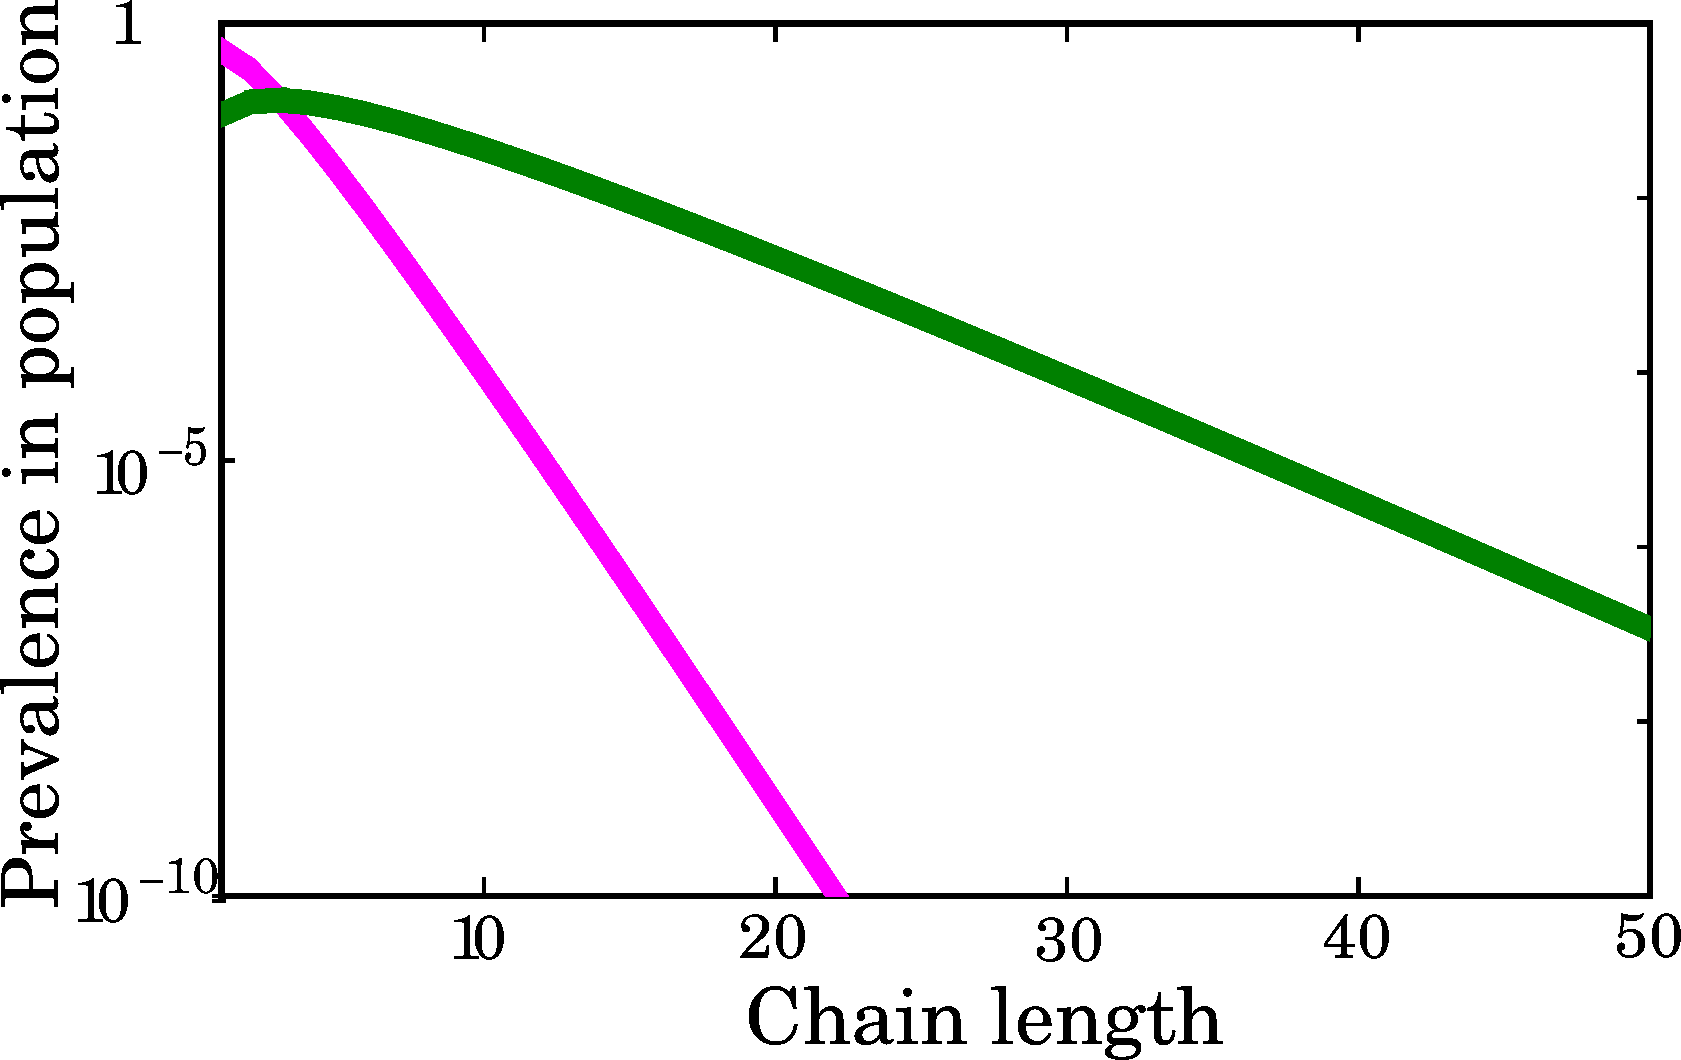
\includegraphics[width=\columnwidth]{pictures/flory2.pdf} 
  \caption{\textbf{Polymerization processes lead to mostly short chains.}  Spontaneous 
polymerization processes typically lead to the Flory distribution of chain lengths. 
Green line gives $\langle  l \rangle= 6$, magenta one corresponds to $\langle l \rangle=2$}
  \label{fig:flory}
\end{figure}

The Flory distribution is a good model for various known prebiotic syntheses of peptide and 
nucleic 
acid chains.  Figure~\ref{fig:some_flory} shows that the Flory model fits known length 
distributions from various prebiotic syntheses (sometimes data is fit to an exponential law, 
$f(a)\propto 
const^l$, which is slightly simpler but nearly identical in form 
~\cite{nowak2008prevolutionary,Derr2012}).  So, since experiments on a.a. polymerization and 
prebiotic chemistry appears to give submillimolar or submicromolar 
concentrations~\cite{Stribling1987,Huber1998,Aubrey2009,Kanavarioti2001,Lazcano1996} of monomers, 
longer chains have been expected to be present in negligible concentrations.  The Flory problem is 
not solved by improving the catalyst~\cite{Derr2012}. 
One needs 
a substantial change in the dynamics of the system to change the steady state distribution. 
Improving the catalyst, on the other hand, changes $a$ in (\ref{eq:flory}), but doesn't affect the 
exponential nature of the law.

\begin{figure}[h!]
  \centering
  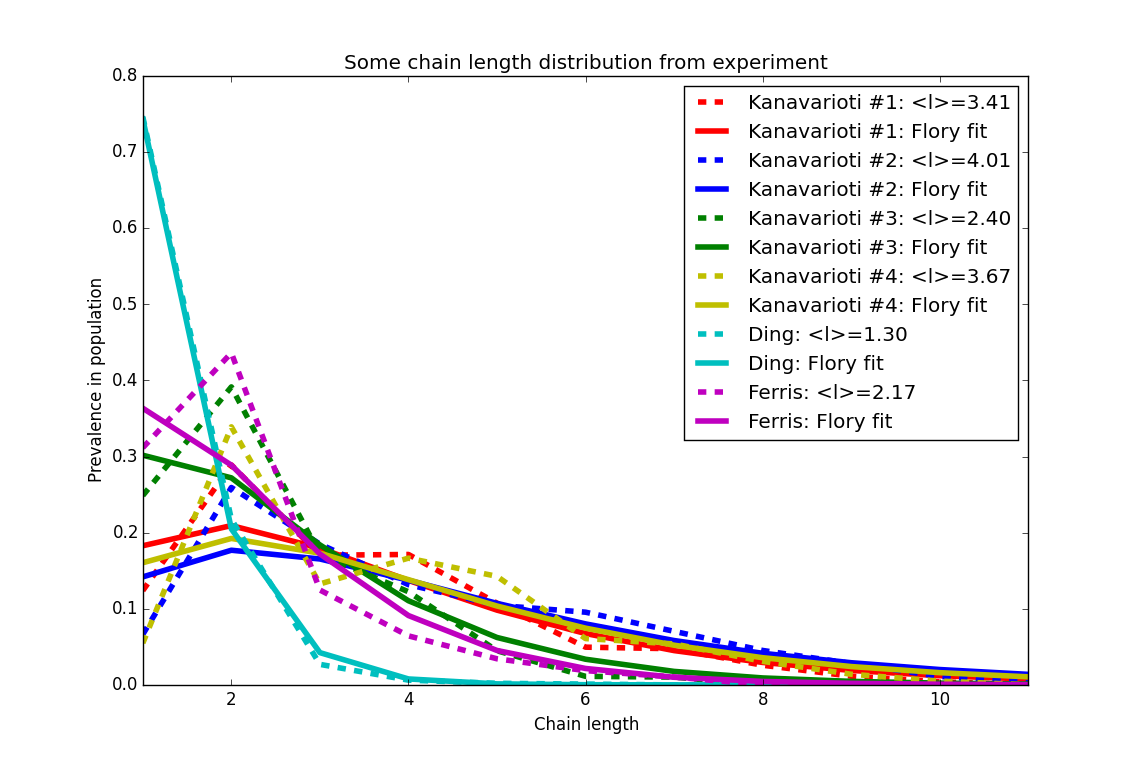
\includegraphics[width=\columnwidth]{pictures/some_flory.png} 
  \caption{\textbf{Prebiotic syntheses of peptides and nucleic acids lead approximately to the 
Flory length distribution.}  Data 
points: red -- Kanavarioti~\cite{Kanavarioti2001}, cyan -- Ding~\cite{Ding1996}, 
magenta -- Ferris~\cite{Ferris1999}}
  \label{fig:some_flory}
\end{figure}


\section{Proposed mechanism: Short $HP$ chains fold in water and catalyze the elongation of other 
$HP$ chains}

 We believe that some puzzles of prebiotic chemistry might be resolved by recognizing the 
 special properties of $HP$ polymers.  $HP$ polymers are copolymers in which the monomer units can 
be categorized as hydrophobic ($H$) or polar ($P$), in particular sequences.  Proteins are 
present-day $HP$ polymers: the 20 amino acids can be divided into the two classes, $H$ or $P$.  In 
$HP$ polymers, the sequence patterning of the $H$ and $P$ monomers lead to a solvation-based 
encoding of sequence-structure relationships~\cite{Chan1991}.  The 2D HP model is the model of 
choice for studying folding-related properties of random sequences, because the full sequence and 
conformational spaces can be studied by exhaustive enumeration, without assumption or adjustable 
parameters. 

   Here is the overview of the mechanism that is supported by our model simulations below.  
   Suppose that a polymer molecule $A$ folds so that it has exposed hydrophobic monomers on its 
surface.
Such exposed cluster of hydrophobes or ``hydrophobic patches'' are fairly common for real 
life proteins; their locations generally coincide with binding sites of ligands or other 
proteins~\cite{Lijnzaad1996}. They are exploited in recognition, binding of substrates 
and increasing rate of catalysis \cite{MitchellGuss1983,Lijnzaad1996,VanEe1997,Witt1998}. For 
example hydrophobic patches on the surface of lipases serve as initiation sites; 
hydrophobic tail of a surfactant interacts with the patch first~\cite{VanEe1997}. Hydrophobic 
patch 
in Cytochrome-c Oxidase one the other hand doesn't serve as recognition element but increases 
$k_{cat}$~\cite{Witt1998}. A survey of hydrophobic patches on the surface of 112 soluble, 
monomeric 
proteins\cite{Lijnzaad1996} showed that the largest patches average around $400$\textit{\AA}$^2$ 
but can range from $200$ to $1,200$\textit{\AA}$^2$.

 We propose thus that exposed hydrophobes on the surfaces of folded $HP$ sequences can serve in a 
similar way as sticky spots for unfolded $HP$ chains with hydrophobic tails and for H monomers; 
see 
Fig. \ref{fig:hp-catalysis}.  Hydrophobic interaction between three of them localizes growing 
chain 
and next monomer and reduces the kinetic barrier of polymerization for the growing chain and an 
$H$ 
molecule. In this mode of interaction, catalysis is very promiscuous and concerned only with 
hydrophobic residues. \red{A recent study~\cite{Tonddast-Navaei2015} showed that modern days 
proteins also experience a certain degree of promiscuity when it comes to protein-protein 
interactions with typical protein having nearly a dozen protein interaction partners and nearly 3/4 
of its surface having geometrical properties that are amenable to interactions. These sites of 
interaction are enriched in hydrophobes. }

A typical hydrophobic interaction is $1-2kT$.  
Consequently chain $A$ is a 
catalyst that provides a hydrophobic landing pad and reduces activation energy by 3-4 hydrophobic 
interactions, thereby increasing the polymerization rate around $ 100$-fold.  Of course, this rate 
enhancement is much smaller than the 
$10^7$-fold of modern ribosomes~\cite{Sievers2004a}. Nevertheless, it gives a conceptual basis for 
how peptide-bond formation rate enhancements might have had their prebiotic beginnings.  

Our studies 
below lead to two main conclusions.  First, even random processes that synthesize random $HP$ 
sequences will lead to some selection that can concentrate some sequences and structures over 
others.  Second, some folded $HP$ sequences can have primitive catalytic and autocatalytic 
abilities, based on their exposed hydrophobic surfaces, whereby certain chains can help to 
polymerize other chains.  So, the folding and binding sites of $HP$ polymers could explain how 
prebiotic chemistry might escape the Flory Problem.
   
   \begin{figure}[h!]
  \centering
  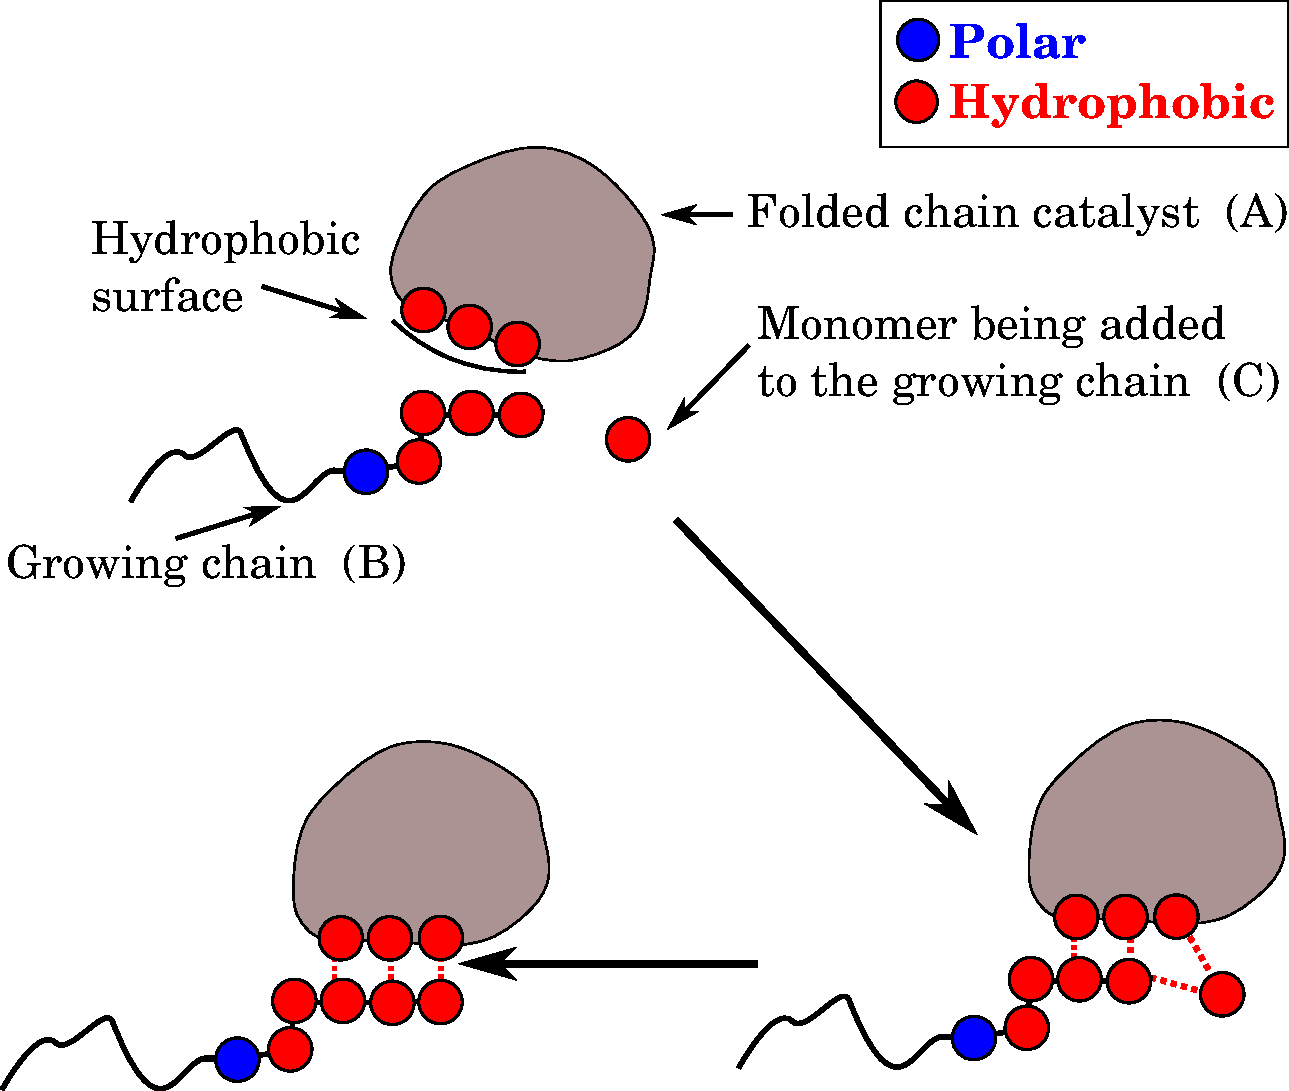
\includegraphics[width=0.9\columnwidth]{pictures/hp-catalysis.pdf} 
  \caption{\footnotesize{\textbf{Some HP foldamers have hydrophobic patches, which serve as 
landing pads that can catalyze the elongation of other HP chains.}  Chain $A$ folds and exploses 
hydrophobic monomers on its surface.
 That serves as a sticky spot for another $HP$ molecule $B$, in addition to an $H$ monomer $C$.  
This localization action reduces the barrier to the polymerization of chain $B$ to monomer $C$.  If 
the landing pad is 3-4 hydrophobic residues, this localization can reduce the barrier by 
$100$-fold, the sticking energy.}}
  \label{fig:hp-catalysis}
\end{figure} 

 $HP$ polymers have been studied extensively as a model for the folding and evolution of 
 proteins~\cite{lau1989lattice,Chan1991,Miller1995,Yue1995,agarwala1997local}.  Such studies have 
shown that stably folded structures of proteins to a large extent can be explained by binary 
pattern 
of polar and hydrophobic residues and do not require knowledge of specific interresidue 
contacts~\cite{Yue1992,Xiong1995,Fisher2011}. A large fraction of the space of random sequences 
can 
collapse into compact structures resembling native proteins~\cite{lau1989lattice}; see 
fig.~\ref{fig:hydro-effect}.  While the 2-dimensional HP lattice model entails obvious 
simplifications, it has the advantages that: (1) it is currently the only model that can explore 
full sequence and conformational spaces, without assumptions or approximations, and (2) it is 
known 
to reproduce key observations on real proteins in 3D.  The reason that the dimensionality is not 
problematic is that the principle physics is in the surface-to-volume ratios of HP chains 
collapsing 
in water, and the 2D model for 12-25-mers in 2D is the same as that of 100-200-mer proteins in 
3D~\cite{Giugliarelli2000}. 
 
  We note that the present model is not particularly intended to be restricted to proteins.  
  RNA molecules are also able to fold in water, indicating differential solvation.  While our 
present model focuses on hydrophobic interactions, it is simply intended as a concrete model of 
solvation, that could more broadly include hydrogen bonding or other interactions.  So, while our 
analysis below is only applicable to foldamers, it is not limited to proteins.
 

\begin{figure}[h!]
  \centering
  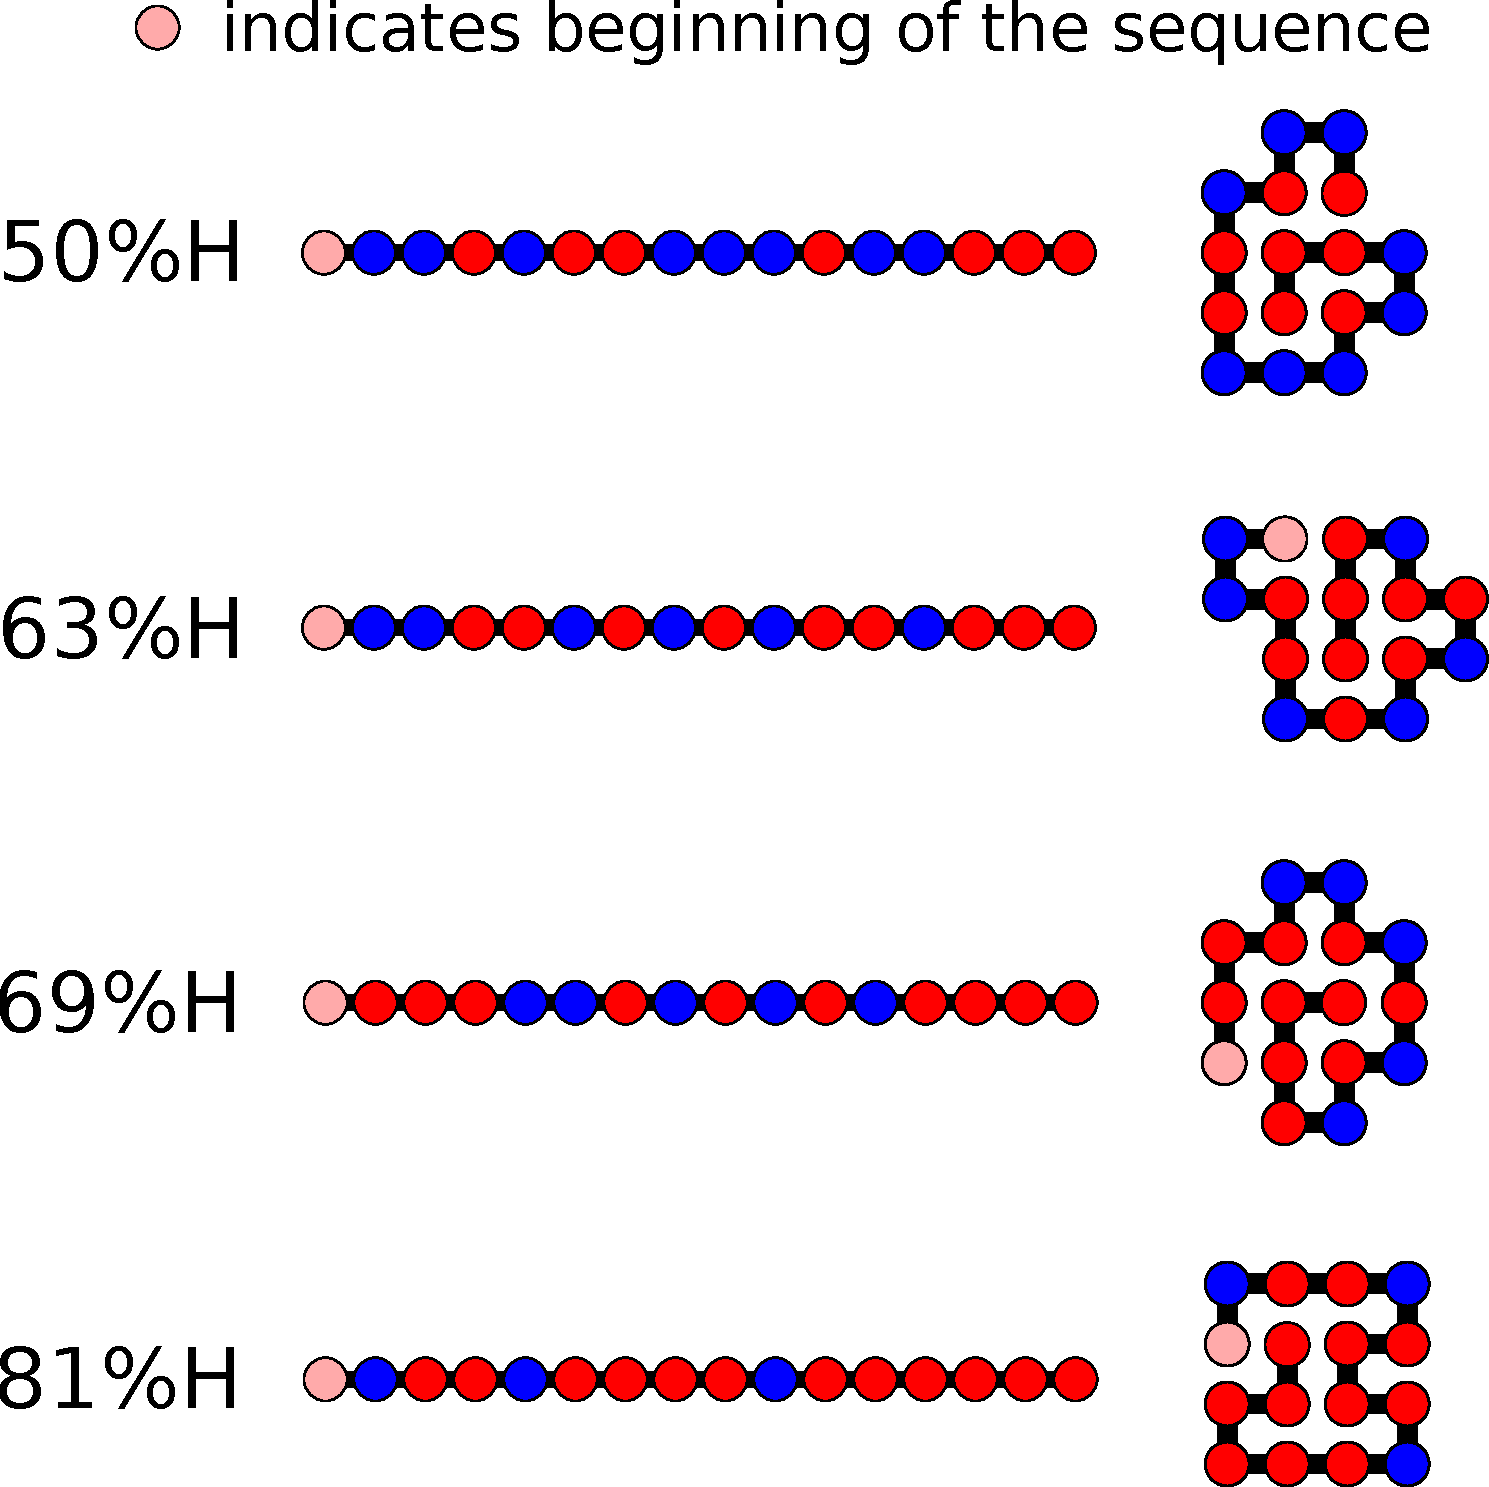
\includegraphics[width=\columnwidth]{pictures/tst-seqs.pdf} 
  \caption{\footnotesize{\textbf{HP sequences that fold to unique native structures in the HP 
lattice model.}}}
  \label{fig:hydro-effect}
\end{figure}


\subsection{The model of $HP$ polymerization kinetics}

 We consider a soup containing a sufficient supply of activated $H$ and $P$ monomers in solution. 
 Activated $H$ and $P$ monomers are supplied by an external source with rate $a$.  Any molecule 
can 
be removed from the system with rate $d$.  A given chain elongates through the 
an addition of a monomer, at rate $\ga$. Without loss of 
generality we define the unit rate by setting $\ga = 1$.  All other rates are taken relative to 
this 
chain growth rate.  We assume all polymers also undergo spontaneous hydrolysis; any bond can be 
broken with rate constant $h$.  

 Now, in addition to this basic polymerization dynamics, we also account for the fact that some 
sequences 
will fold into native HP structures, protecting its hydrophobic core residues from hydrolysis.  It 
is important to note though that, what we call folding doesn't have to be a tight folding, which 
happens in long proteins which went through evolution, but can be merely a molten globule state -- 
something that gives certain stability to the structure.
the standard definition for HP polymers, we regard a chain as folded if it has a unique 
lowest-energy structure.  That is, some sequences have only a single conformation giving a maximum 
number of HH non-covalent contacts.  (Most sequences, in contrast, 
have many low-energy states; we do not count these as folded structures.)  
We use a two state model of folding: chains are either unfolded or folded in 
thermodynamic minimum. 
The conformational energy of the native fold ($E_{nat}$) of any particular folded sequence equals 
the number of hydrophobic interactions ($n_{h\phi}$) $\times$ the energy $E_H$, of one hydrophobic 
interaction, which is known to be $\approx 1-2kT$~\cite{Ghosh2009}:
\begin{equation}
 E_{nat}=n_{h\phi}E_H.
\end{equation} 
This energy differs for different sequences.  Now, given knowledge of $E_{nat}$ for any particular 
sequence, we can readily compute the folding and unfolding rate coefficients from~\cite{Ghosh2009}:
\begin{equation}
 \ln\pt{\frac{k_f}{k_u}}=-\gD G/kT = E_{nat}/kT-N\ln z,
\end{equation} 
for reversible folding, where $z$ is the number of rotational degrees of freedom per peptide bond. 
 

We suppose that chains that fold are prevented from further growth, and also are protected from 
hydrolysis.  This simply reflects that open chains are much more accessible to degradation from 
the 
solvent or adsorption onto surfaces than are folded chains.  Even so, folding in our model is a 
reversible, as it is for natural proteins, so some small fraction of the time even 
folded chains are unfolded, and in that proportion, our model allows them further growth and 
degradation.
 



\subsection{Results: some basic tests of the dynamics of polymerization and folding}

 We performed a computational experiment just to test that this dynamical model leads to the 
 Flory equilibrium distribution.  In this simple test, we excluded folding and catalysis by 
setting 
the hydrophobic energy to $0$. Figure \ref{fig:sim_pure_flory}(a) shows that, as expected, the 
length 
distribution has an exponential tail. Figure \ref{fig:sim_pure_flory}(b) shows populations of 
individual sequences in a randomly chosen realisation of the experiment. For more details see 
Simulations. Experiment 1.

\begin{figure*}[hbt!]
  \centering
  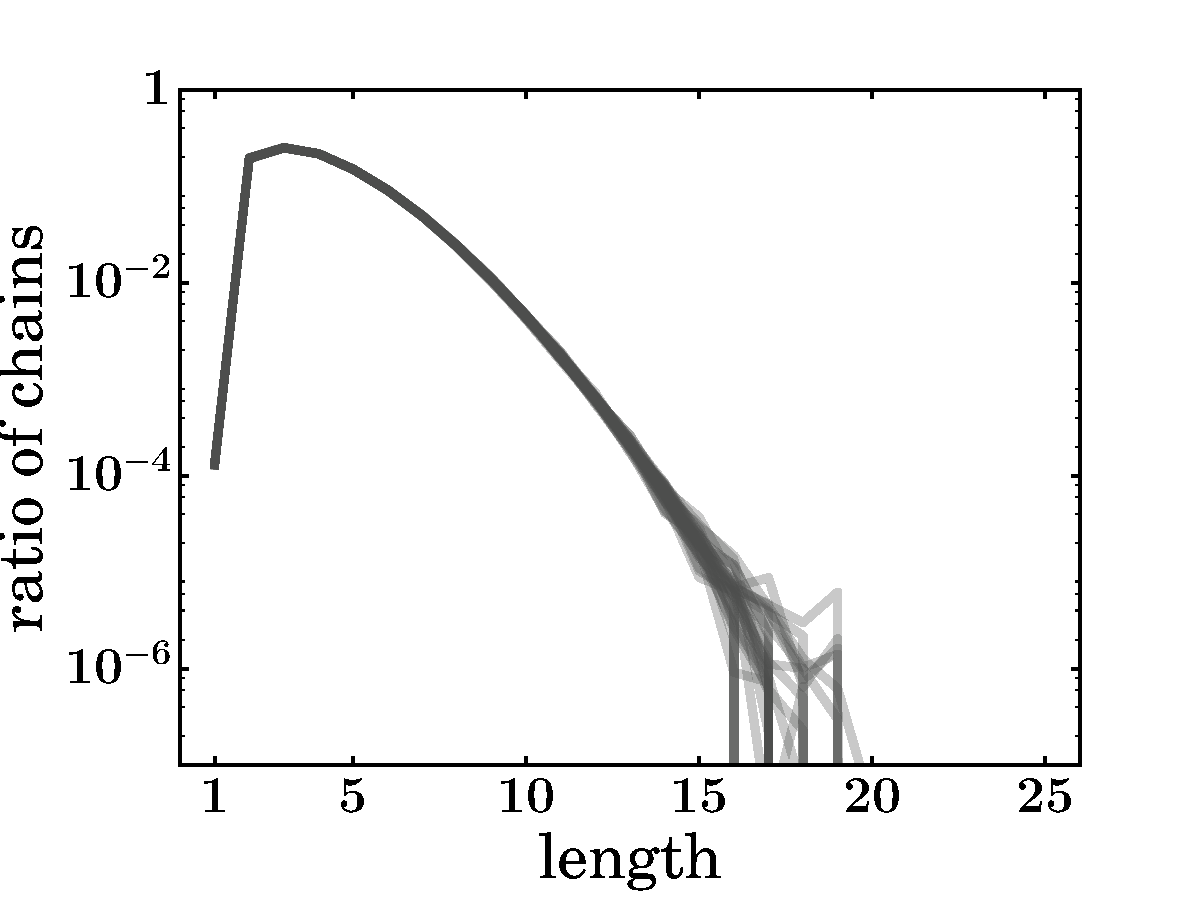
\includegraphics[width=0.45\textwidth]{pictures/distrPlain-many.pdf} (a)
  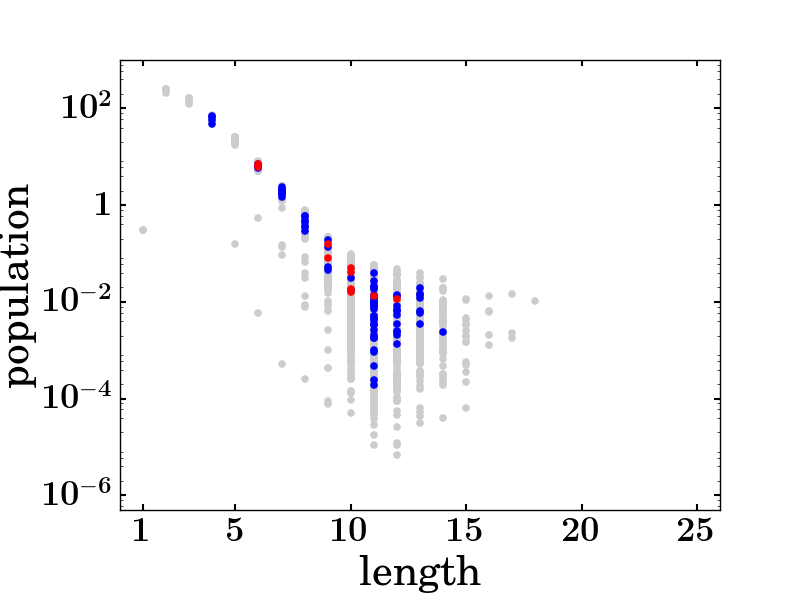
\includegraphics[width=0.45\textwidth]{pictures/scatter01918.png} (b)
  \caption{\footnotesize{\textbf{A.  Reference experiment.  The HP model, treated without folding 
or catalysis, leads to the Flory distribution, as expected.}  Results of the Experiment 1: no 
folding, no catalysis polymerization. This 
is the base case to which we compare all other systems. Each data point is an average of 
$10^6$ time points in the steady state interval. (a) A single line shows the length distribution 
for one simulation run (we run total of 30 simulations). (b) \bf{Some specific sequences.}  
Populations of the individual sequences, based 
on the results of a single simulation run. 
We set $E_h=0$, but still show sequences,which could've fold (if not $E_h=0$) as 
blue, and sequences which could've catalyze as red. As expected, they follow the same distribution 
as other sequences.}}
  \label{fig:sim_pure_flory}
\end{figure*}



\section{Folding alone does not solve the Flory Problem}
Our second computational experiment asks whether HP chain folding alone is sufficient to alter the 
Flory length distribution.  In short, we ask whether the few randomly synthesized sequences that 
happen to fold, which therefore also happen to protect their interior residues from hydrolysis, 
lead 
to changing the Flory length distribution.  Details are in experiment 2; see Simulations. 
Figure~\ref{fig:sim.flory-fold} shows that chain folding alone, of the few foldable sequences, is 
not sufficient to escape the Flory problem of the exponentially diminishing concentrations of 
chains 
with length.  Folding does increase the abundances of some of the folded sequences.  Yet, their 
instances are so rare that they do not alter the distribution.  Thus, folding alone does not 
explain 
how prebiotic polymers escape the Flory Problem.
\begin{figure*}[hbt!]
  \centering
  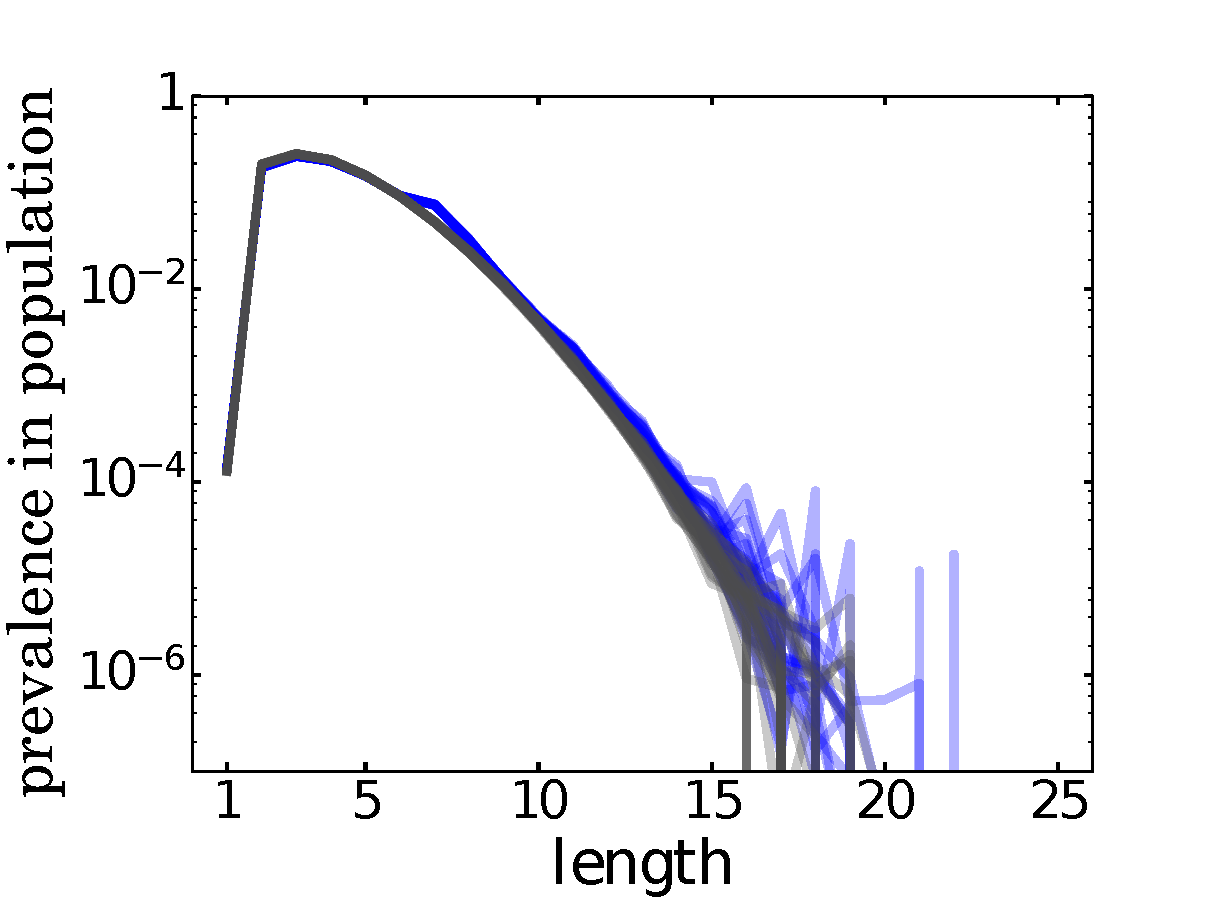
\includegraphics[width=0.9\columnwidth]{pictures/distr-folded-many.pdf} (a)
   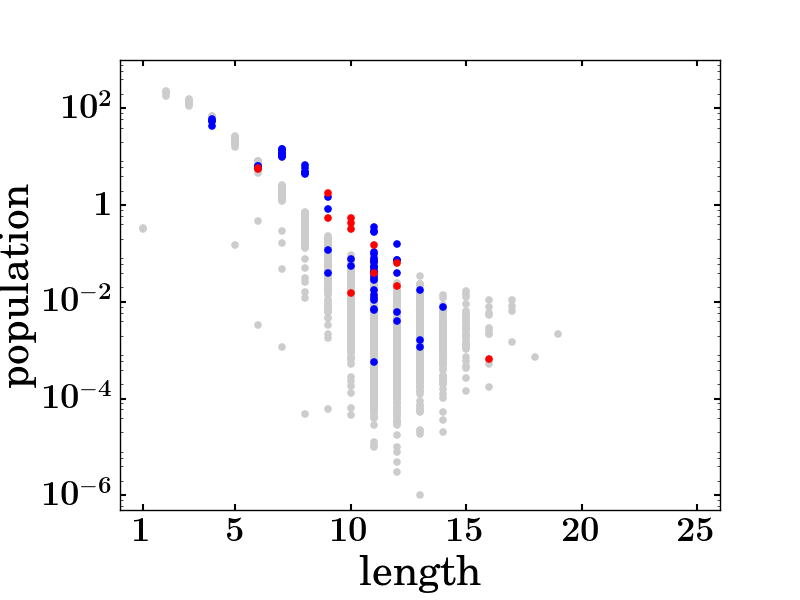
\includegraphics[width=0.9\columnwidth]{pictures/scatter209.png}(b)
  \caption{\footnotesize{\textbf{Experiment 2: HP polymerization, now including folding, but not 
including catalysis.  This, too, only gives the Flory distribution.}  Each data point is an 
average 
of $10^6$ time points in the steady state interval. (a) 
A single line shows length distribution for one simulation run (we run total of 30 simulations). 
Blue lines are result of the Experiment 2, gray ones -- Experiment 1. Addition of folding to the 
basic model doesn't change the nature of distribution. (b) Populations of the individual 
sequences, 
based on the results of a single simulation run. Gray dots -- unfoldable sequences, blue ones -- 
foldable. In this simulation we disallow catalysis, but we still show potential catalysts in red, 
to show, that they behave similarly to regular folders. Foldable sequence have advantage compared 
to unfoldable ones.}}
  \label{fig:sim.flory-fold}
\end{figure*}

\section{Primitive foldamers can also be primitive catalysts}

 In our third experiment, we also accounted for the effect of some HP foldamers to catalyze 
reactions.  Of course, present-day foldamers (proteins and RNA molecules) can catalyze reactions 
very 
efficiently -- including the reaction in the ribosome that synthesizes the peptide 
bond~\cite{Stachelhaus1998}. These modern catalysts have evolved over a long time towards 
exceptional catalytic functionalities.  Of course, prebiotic functionalities are likely to have 
been 
much more primitive.  Our interest here is in how the most primitive catalysts might have begun.  
Precision and complexity isn't a requirement for peptides to perform biological function. Studies 
show that folded proteins generated from random libraries can sustain the growth of living 
cells~\cite{Fisher2011} and specific binding actions between those random peptides and small 
molecules are not 
rare~\cite{Cherny2012}. These findings imply that some primitive foldamers could have had some 
primitive catalytic capability.  The unique power that foldable molecules have for catalyzing 
reactions -- in contrast to 
other nonfoldable polymeric structures -- is that foldamers lead to precisely fixing atomic 
interrelationships in relative stable ways over the folding time of the molecule.  It resembles a 
microscale solid, with the capability that substrates and transition 
states can recognize, bind, and react to those stable surfaces. For example, serine proteases 
utilize a catalytic triad 
of 3 amino acids.  So, foldability in some type of prebiotic polymer, could conceivably have had a 
special role in allowing for primitive catalysis.  Here, we use a toy model to capture that simple 
idea, namely that a folded polymer can position a small number of residues in a way that can 
catalyze a reaction. 


\subsection{How chain elongation is catalyzed}

For  the foldable $HP$ sequences with exposed hydrophobic patches the same force that folds them 
by forcing $H$ monomers inside will attract another hydrophobes from the solution. 
If the exposed patch is long enough, then it can serve as a landing pad for a growing sequence and 
hydrophobic monomer, thus holding both together and lowering the activation barrier for the 
polymerization reaction. Therefore catalysis rate are proportional to the exponent of hydrophobic 
energy $E_H$ and number of contacting 
hydrophobes $n_c$: $\ga\cdot\exp(E_{H}\cdot n_{c}/kT)$(see figure \ref{fig:fold-cat}).  
For the modeling we set minimum size of the landing pad to be 3. Thus catalysts facilitate $\cdots 
HH$ to 
$H$ connections. So every polymer, which has $HHH$ in its sequence can benefit from catalysis. 

\begin{figure}[htb!]
  \centering
  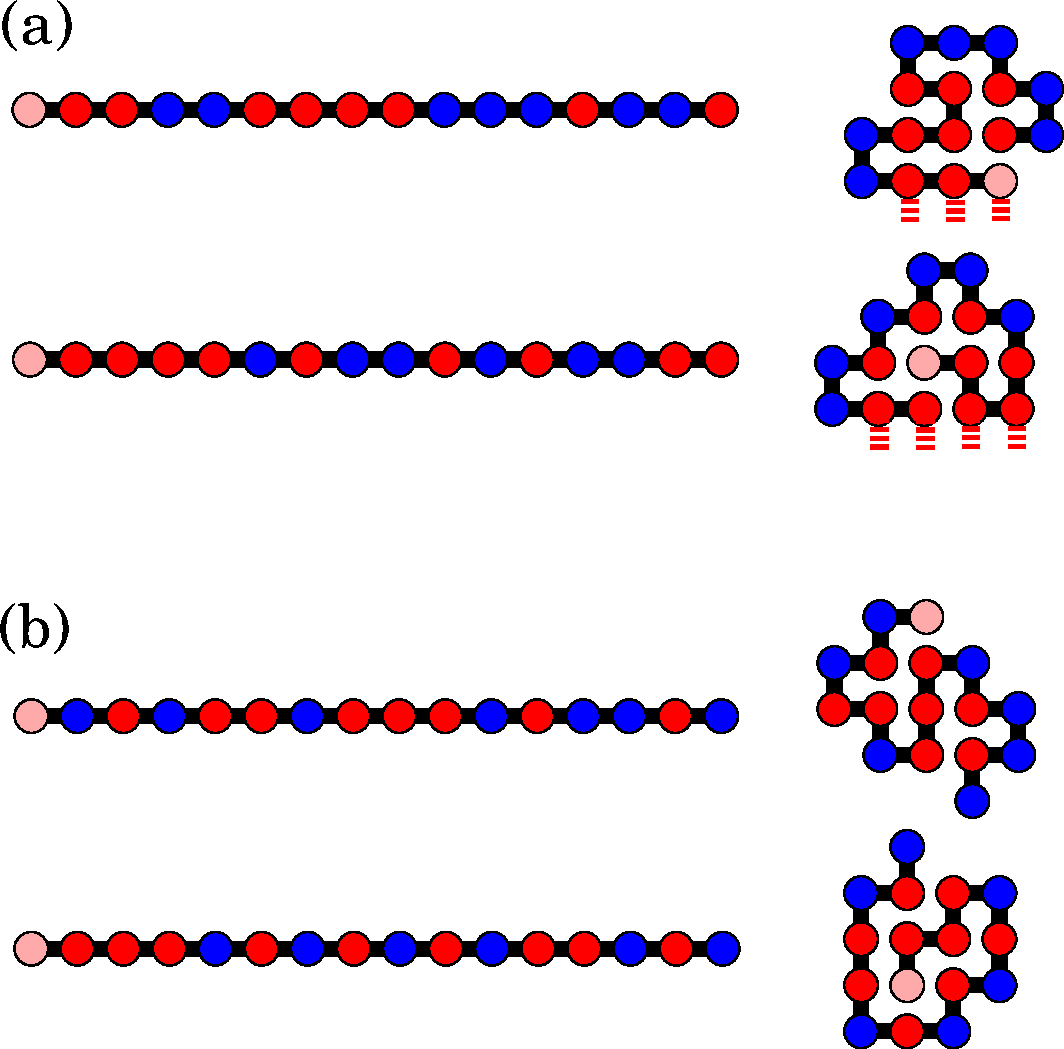
\includegraphics[width=\columnwidth]{pictures/fold-cat.pdf} 
  \caption{\footnotesize{\textbf{(a) HP lattice chains that are found to be in the autocatalytic 
set: they fold and catalyze the elongation of each other.  (b) HP foldamers that are not 
catalysts.}  Most chains are not catalysts, but the size of the autocatalytic set is 
non-negligible; see Fig.~\ref{fig:hp-statistics}.}}
  \label{fig:fold-cat}
\end{figure}

 At this point, we note what our model is, and what it is not.  Our model is not intended as an 
 accurate atomistic depiction of a real catalytic mechanism.  It is a coarse-grained toy model, of 
which there will be variants.  The mechanism we explore here is the translational localization of 
the two reactants, polymer $B$ and monomer $C$, in the chain extension reaction.  And, while this 
model is 2-dimensional, extensive previous studies have shown that it captures many important 
principles of folding and sequence-to-structure relationships.  At the present time, this type of 
model is the only unbiased, complete and practical way to explore plausibilities of physical 
hypotheses such as the present one.


\subsection{Modeling shows that HP foldamer-catalysts can solve the Flory Problem}

Figure~\ref{fig:sim.flory-fold} shows the results of simulations, now allowing for both the 
folding of all HP sequences, according to the rules of the HP model, and allowing for catalysis 
based on all those foldamers that have three $H$ monomers on their surfaces in their unique native 
folded states (see SI for details). Presence of catalysis in the system skews the distribution 
significantly. This distribution is fairly stable towards hydrolysis and dilution
parameters. It allows for 1 order of magnitude change in those parameters without significant 
change in the behavior of the system.

This figure represent one of the key finding of this paper: a simple physical mechanism, such as 
hydrophobic interaction is capable of generating autocatalytic sets of non-trivial structure (for 
details see in Discussion), which despite the initial weak catalytic forces of 
interaction ($E_h\approx 1-2kT$) over time reaches the ability to dominate population. As it's 
clear from the figure \ref{fig:stats-scatter-018}(a) this mechanism also allow for solution of the 
Flory 
problem.

Figure\,\ref{fig:stats-scatter-018}(b) show populations of individual sequence as function of 
their 
length. Colors represent type of the sequence: red -- for autocatalysts, blue -- for foldable, 
gray 
-- for the rest. The distribution inside the length, as one can see is drastically different 
compared to the case with folding only and without folding at all. For those cases, populations 
are clustered near average -- the typical $n$-mer is close to mean. When we introduce catalysis, 
there is no typical member anymore, there are many (often more than  50\% of all $n$-mers) 
sequences with very low populations and few with very high ones. In fact, the distribution within 
length is polynomial. Autocatalysts alone constitute a minority of the sequence space ( 
$\approx 
0.6\%$ 
of all the represented in the experiment sequences; foldable but inactive sequences occupy 
$\approx 
2.3\%$, regular sequences -- $\approx97.1\%$), however their contribution to the total mass is 
impressive: 
$\approx 15.7\%$; inactive folders -- $\approx 29.2\%;$ regular sequences $\approx 55.1\%$. 
Moreover, the longer the chain length, the higher the input of autocatalysts into total mass of 
that length (see figure \ref{fig:biomass}). This happens first of all due to increasing number of 
autocatalysts among longer sequences (see fig.\ref{fig:hp-statistics} and also due to the fact 
that 
folding along isn't capable of reaching longer chains. While at the shorter chains preservation 
from hydrolysis by means of folding is enough at longer chains active influence of catalysis is 
necessary.
\begin{figure}[hbt!]
  \centering
  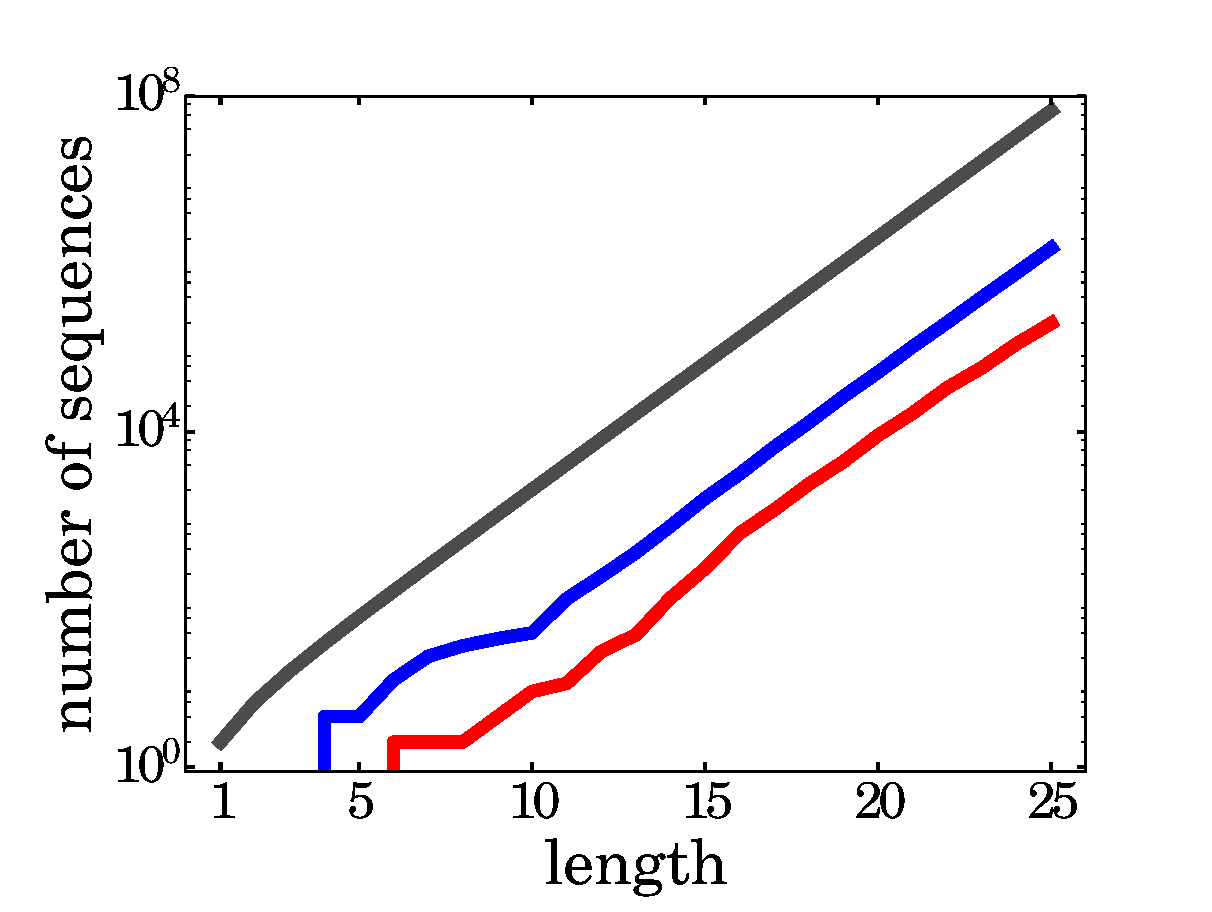
\includegraphics[width=\columnwidth]{pictures/hp-statistics.pdf} 
  \caption{\footnotesize{\textbf{The number of all HP sequences grows exponentially with chain 
length (gray).  The number of foldamers (blue) and foldamer catalysts (red) also grow 
exponentially.}}}
  \label{fig:hp-statistics}
\end{figure}


\begin{figure*}[htb!]
  \centering
  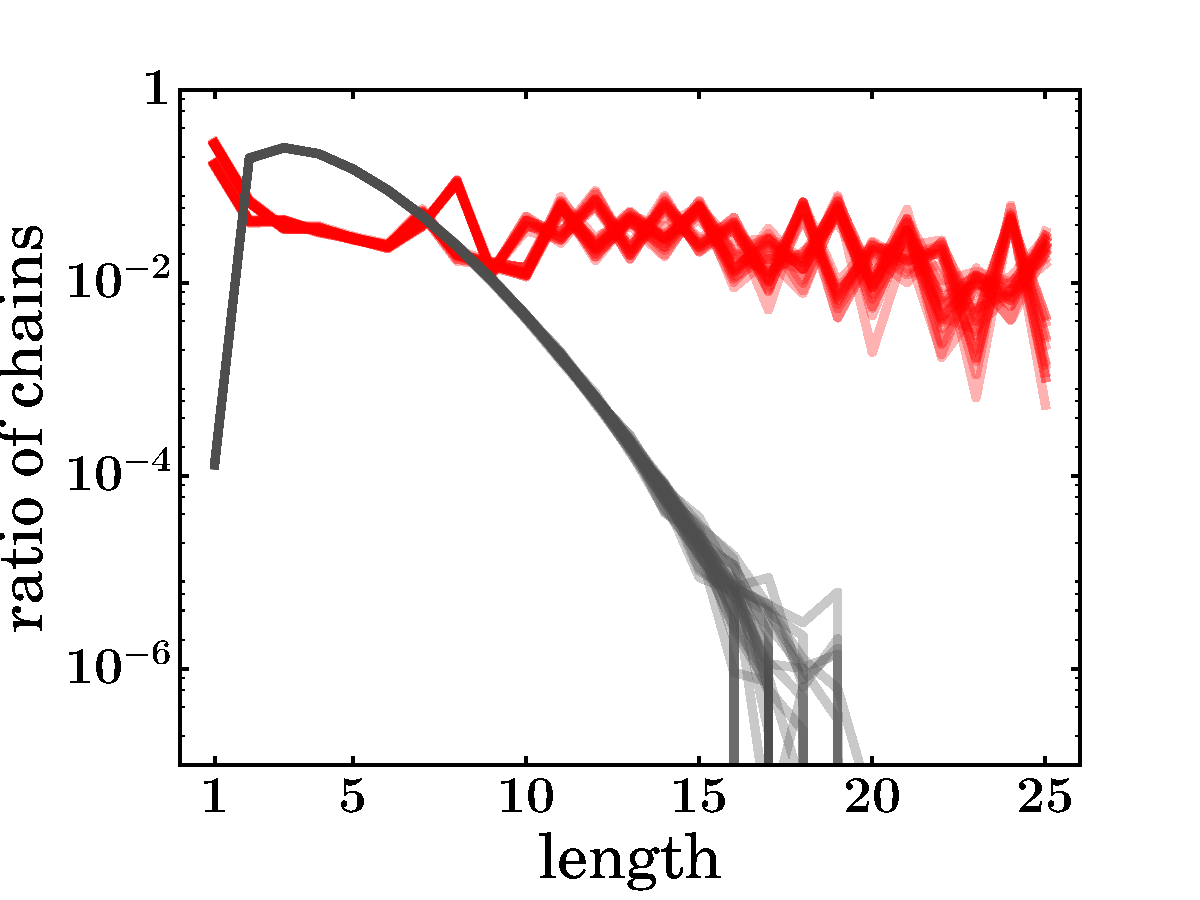
\includegraphics[width=0.9\columnwidth]{pictures/distrHP-plain-many.pdf}(a) 
  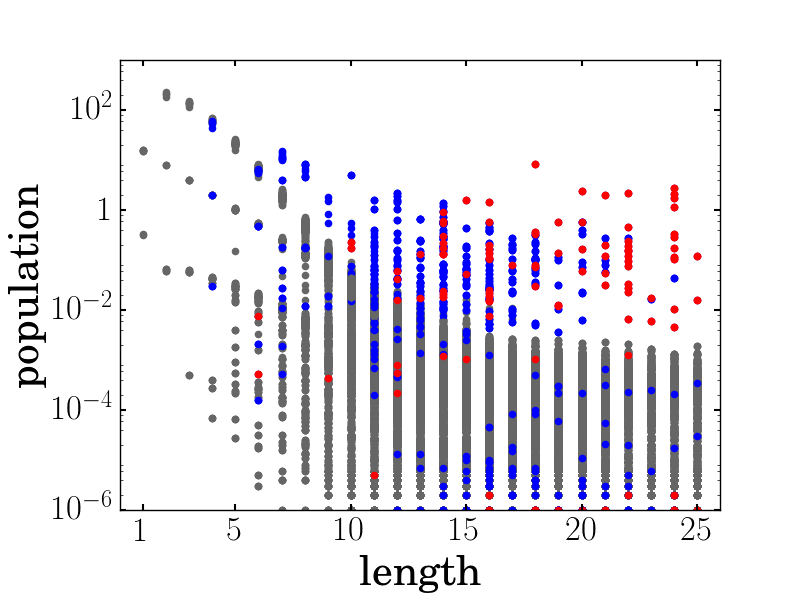
\includegraphics[width=0.9\columnwidth]{pictures/scatter1837.png}(b) 
  \caption{\footnotesize{\textbf{Experiment 3: Because some HP chains are foldamer-catalysts, it 
bends the Flory curve, giving an amplification of longer chains.}  Each data point is an average 
of 
$10^6$ time points in the steady state interval. (a) Gray lines represent polymerization without 
folding or catalysis. Red ones corresponds to a simulation run with folding and catalysis. A 
single 
line shows length distribution for one simulation run (we run total of 30 simulations). For 
details 
of simulations see section Simulations, Experiment 3. (b) Populations of individual sequences are 
shown as 
functions of their length. Autocatalytic sequences are shown in red, sequences that can fold but 
cannot act as  catalysts -- in blue, and all the other sequences in gray. Lower limit of $10^{-6}$ 
is due to computational precision -- there are $10^6$ time steps over which we calculate average 
to 
get a point on the graph. Therefore the minimum possible population correspond to the case when 
sequence appeared only for one time instance. The data is an example based on one simulation}}
  \label{fig:stats-scatter-018}
\end{figure*}

\begin{figure}[h!]
  \centering
  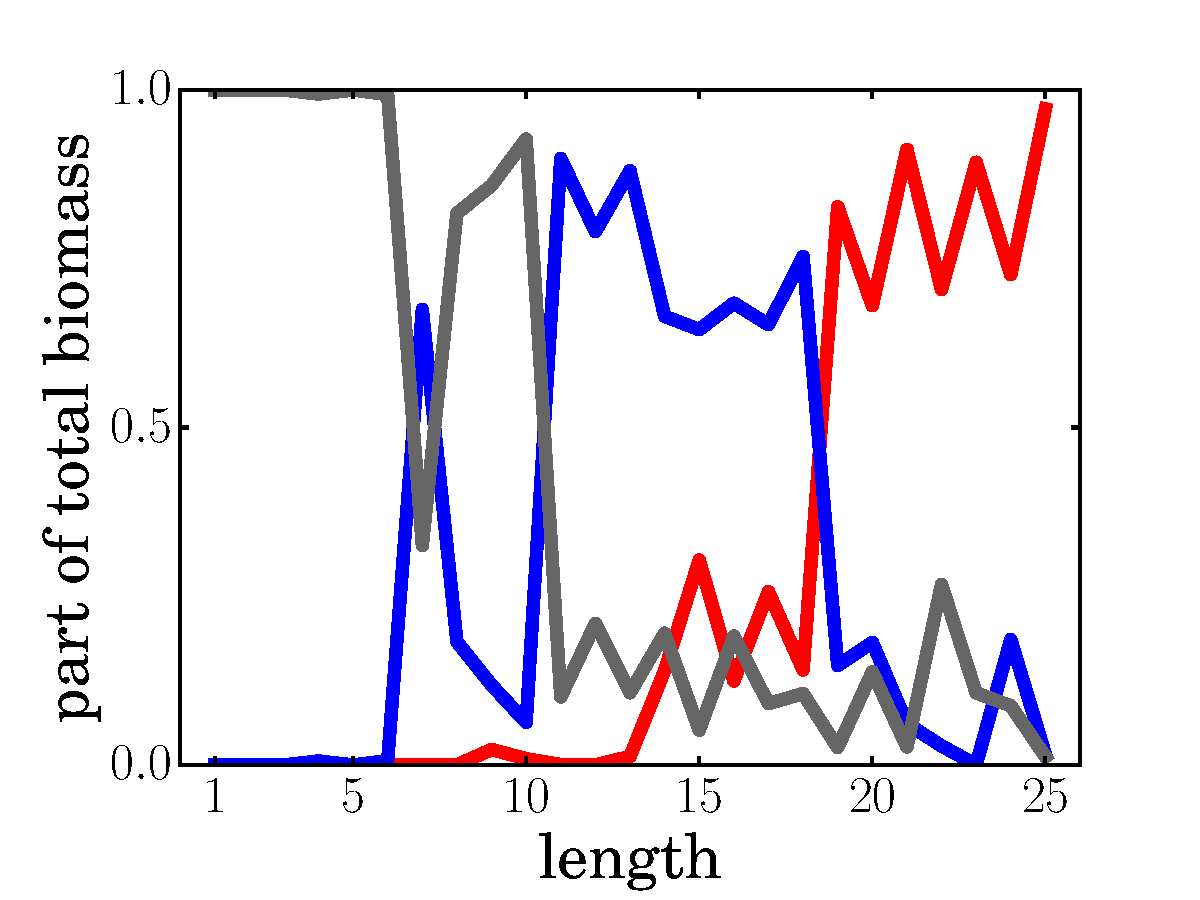
\includegraphics[width=\columnwidth]{pictures/biomass.pdf} 
  \caption{\footnotesize{A single red line shows what ratio of the biomass of the 
given length is due to autocatalysts for a single simulation run. Each data point is an average of 
$10^6$ time points in the steady state interval. Black line is a median over 30 simulations }}
  \label{fig:biomass}
\end{figure}

Average hydrophobicity of those sequences which dominate their length is $68\%$ (average is 
taken over 30 simulation runs in Experiment 3).
Figure \ref{fig:mainplayers} illustrates what kind of sequences and structures dominate. Panel 
(a) shows one top chain for every length, where autocatalysts have significant input in the 
total populations. They are shown as triangles, with the color of triangles 
corresponding to the hydrophobicity of the chains. The folds of these top sequences are shown in 
(b) panel of the figure. For the most of the cases in this particular simulation have 
$k_cat\approx400$. For different values of hydrophobic energies $E_h$ those values might range 
from $50-50,000$, with effect of autocatalysis being visible. These sequences have tendency to be 
main contributors into the total population of the polymers of their length (gray line shows sum 
of all the populations of all the sequences as function of length). They are also notably far from 
the median population (green line), with some exceptions: there are autocatalysts among 11-14 
mers, but none of them managed to emerge above average and aren't shown on the picture.
\begin{figure}[h!]
  \centering
  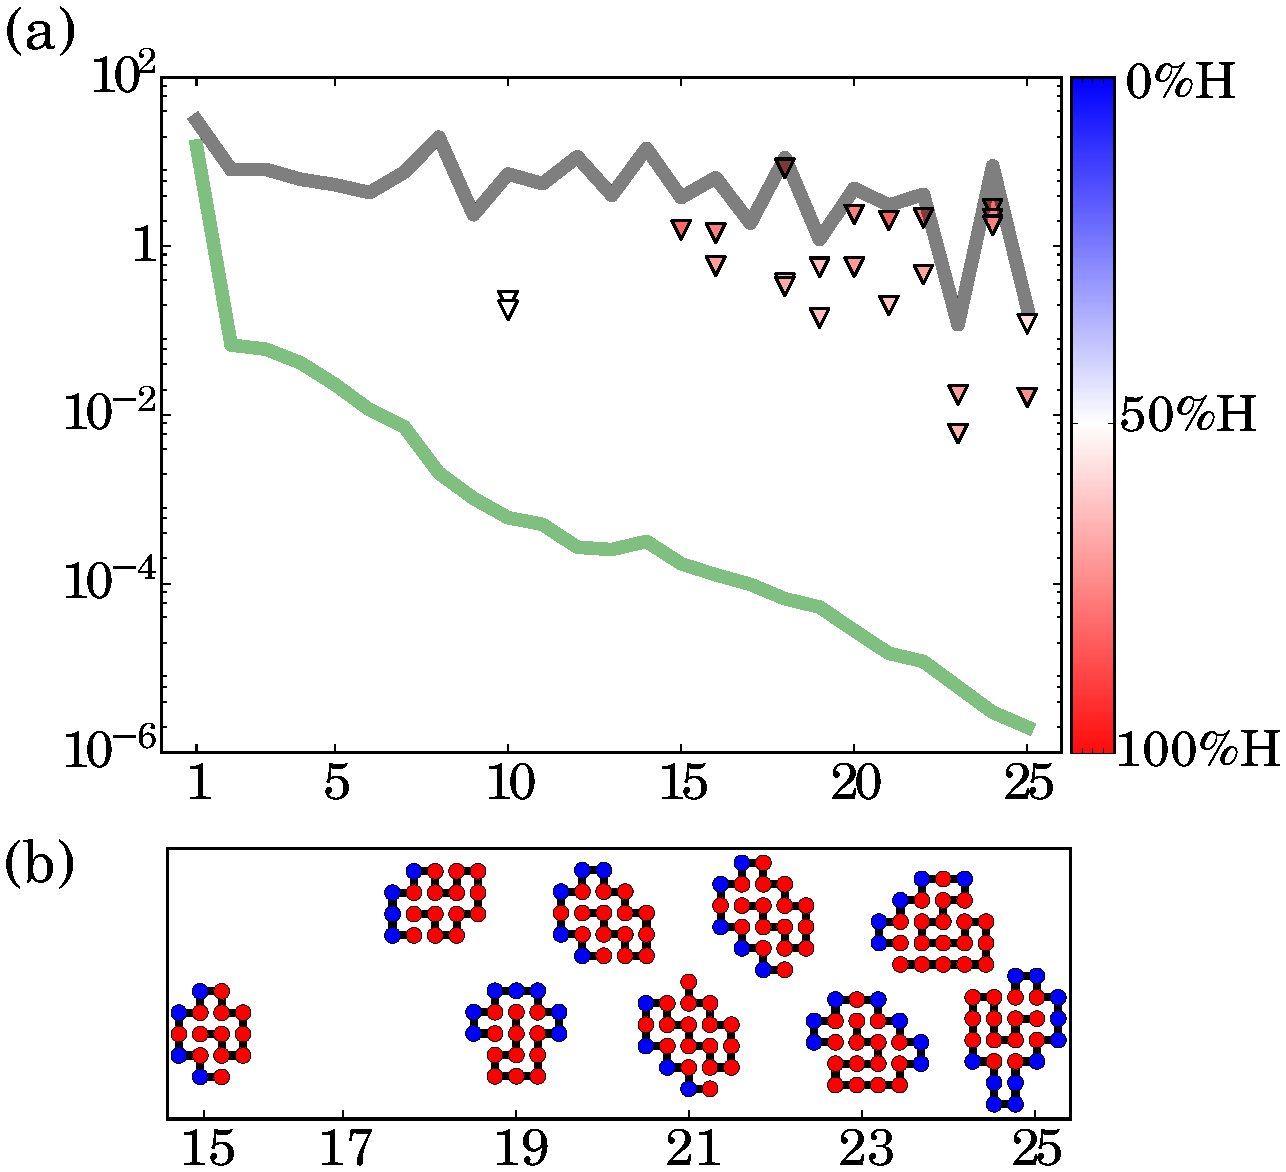
\includegraphics[width=\columnwidth]{pictures/mainPlayers.pdf} 
  \caption{\footnotesize{(a) Show several top autocatalytic sequences. Their color indicate their 
hydrophobicity with more red being more hydrophobic. Green line -- is the median of the 
populations. Top autocatalysts always have several orders higher population, which is generally 
constitutes bulk part of the given length biomass. Biomass as function of length is shown in 
gray. (b) Shows top sequences and their fold for the longest length}}
  \label{fig:mainplayers}
\end{figure}

 



\section{Discussion}
\label{sec:evolution}
 It has been recognized that life's origins require some form of 
autocatalysis~\cite{Kauffman1986,Dyson1985,Eigen1978}.  But, what molecular structural mechanism 
might explain it?  Here, we find that autocatalysis is inherent in the following process (see 
Figure \ref{fig:kinExamples}):  HP polymers 
are synthesized randomly; a small fraction of those HP polymers fold into relatively stable 
compact 
states; a fraction of those folded structures provide relatively stable `landing pad' hydrophobic 
surfaces; those surfaces can help to catalyze the elongation of other HP molecules having foldable 
sequences.

\begin{figure}[h!]
  \centering
  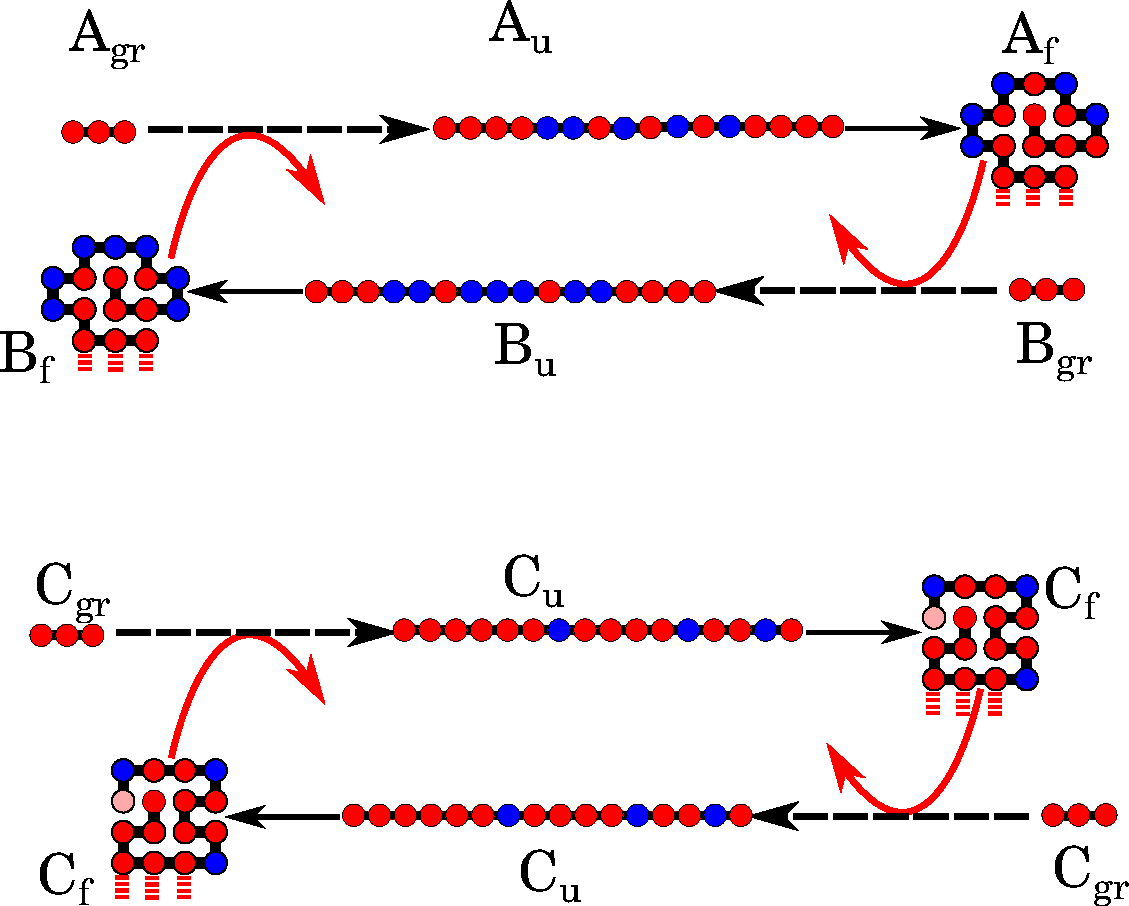
\includegraphics[width=0.9\columnwidth]{pictures/catalysis-kinEx-all.pdf}
  \caption{\footnotesize{Two examples of cross and autocatalytic interaction naturally embedded in 
HP-polymers dynamics. Dashed arrows (\textbf{-\,-\,-}) are shorten representation of multiple 
reactions of chain among which there are $\cdots HH - H$ catalyzed reactions. Catalysis is 
represented by red solid arrows (\red{\textbf{\textemdash}}). Solid black lines 
(\textbf{\textemdash}) are folding reactions. Chains, which we call ``autocatalytic'' experience 
catalysis during one (or more often several) of the steps of elongation. Then, when they reach the 
length at which they can fold ($A_u,\, B_u,\, C_u$), they fold and serve as catalysts them selves 
($A_f,\, B_f,\, C_f$). Mutual catalysis cat happen between different sequences (here A and B) and 
between different instances of the same sequence (here C).}}
  \label{fig:kinExamples}
\end{figure}

 The HP model allows for unbiased counting of sequences that do fold, don't fold, or fold and have 
a potentially catalytic hydrophobic landing pad.  A non-negligible fraction of all possible HP 
sequences fold to unique structures ($2.3\% $ for lengths up to 25-mers). The fraction of all 
possible HP sequences that have catalytic surfaces (as defined above) is $12.7\%$ of foldable 
sequences, or $0.3\%$ of the whole sequence space.  These ratios remain relatively constant with 
chain length, at least up to 25-mers; see figure \ref{fig:hp-statistics}.  This and successful 
designs of foldable, biologically active proteins based on the HP folding rule~\cite{Murphy2015} 
suggests that folding in HP polymers is not rare.  
 
  The present model provides an experimentally testable prediction for what early 
  polymer sequences could be autocatalytic, and provides a structural and kinetic mechanism for 
their action.  This model also provides a view about how selection and diversity may be related, 
and may be evolvable, arising from chain syntheses that are otherwise random.



\section{Materials and methods}\label{sec:mat}
\subsection{Simulations}\label{sec:mat-sim}
To test our hypothesis we performed direct stochastic simulations on several sets of parameters. 
We 
used the expandable partial propensity method (EPDM)~\cite{Guseva2016b}.
\footnote{C++ library and description can be found here: https://github.com/abernatskiy/epdm}. 
Stochastic simulations keep track of each 
molecular specie in the system. However simulations are limited due to computational reasons. 
First of all we have to explore conformational space of every polymer. This task is NP-hard (we 
use 
HPSandbox algorithm\cite{lau1989lattice,Dill2008} \footnote{Python implementation and description 
can be found here: http://hp-lattice.readthedocs.org/en/latest/}), so we had to limit 
maximum chain lengths to 25. We also try to keep total number of species in the low thousands, to 
limit computational costs. We do it by introducing dilution parameter $d$: molecules are being 
removed from the system with probabilities $\propto d$. 
This either can mimic a protocell splitting and loose of materials due to it or in the case when 
system isn't bounded by any borders the fact that some molecules will diffuse away. Total number 
of 
molecules varies from simulation to simulation, 
however it mostly holds in the region $10^2-10^4$.

We start our simulations with a small pool of monomers, usually below 100 molecules. 
\begin{itemize}
 \item Monomers can be react with each other and with polymers to produce polymerization reaction 
with rate 
$\ga = 1$
\begin{equation}
 1\mbox{-mer}+n\mbox{-mer} \xrightarrow{\ga} (n+1)\mbox{mer}
\end{equation}
\item These monomers are being imported in the system. with rate $a\gg1$. It is safe to assume 
that 
we would have enough monomers in the system and import of monomers wouldn't be a bottleneck of 
reactions chain. Therefore we explore big values of $a\propto 10^3\ga$
\begin{equation}
 \emptyset \xrightarrow{a} H\,\,\mbox{or}\,\,P
\end{equation}

\item Hydrolysis has constant rate $h$ per bond. Half-life time of hydrolysis bonds in neutral 
conditions and temperatures around room temperature are on the order of hundreds of 
years\footnote{Hydrolysis rate constants of oligopeptides in 
neutral conditions are of the order of $10^{-11}-10^{-10}$: $1.3  10^{-10} M^{-1}s^{-1} $ 
for benzoylglycylphenylalanine ($t_{1/2} = 128 y$)\cite{Bryant1996}, $6.3  10^{-11} M^{-1} s^{-1}$
($t_{1/2}=350 y$) for glycylglycine and $9.3 10^{-11}M^{-1} s^{-1}$ for glycylvaline
\cite{Smith1998}.}. We test hydrolysis rate constants to be about $0.01-1$ of polymerization rate 
constants. This way we account for polymerization conditions, which happens on the order of days 
to years.
\begin{equation}
 n\mbox{-mer} \xrightarrow{h} l\mbox{-mer}+(n-l)\mbox{-mer}
\end{equation}



\item Dilution parameter $d$ mimics cell division and loss of the matter because of that. 
This parameter also serves utilitarian role of limiting total population of the cell. We explore 
valued of $d$ from $\propto 0.01\ga$ to $\propto 1\ga$. Given values of $a$ we'll explore various 
populations from $\propto 10^2$ to $\propto 10^4$ polymers per 
cell.
\begin{equation}
 \mbox{anything} \xrightarrow{d}\emptyset
\end{equation}


\item Folding and unfolding reactions happen very quickly with 
the unfolding rate constants of $k_f\gg k_{u}\gg\ga$. 
\begin{equation}
\begin{split}
 \mbox{folded chain}&\xrightarrow{k_u}\mbox{unfoled chain}  \\
 \mbox{unfoled chain}&\xrightarrow{k_f}\mbox{folded chain}
\end{split}
\end{equation}
The folding rate constant taken 
from~\cite{Ghosh2009}:
\begin{equation}
 \ln\pt{\frac{k_f}{k_u}}=-\gD G/kT = E_{nat}/kT-N\ln z,
\end{equation} 
 where $z$ is the number of rotational degrees of freedom per peptide bond.
 $HP$ model itself predicts only equilibrium constant, but not folding/unfolding rates.
 For those we had to rely on statistical models based on data on $k_f,\,k_u$ for 3D real life 
proteins~\cite{Ghosh2010,Dill2011}.
It helps that for our story actual precise numbers for these rates aren't necessary -- population 
of folded vs unfolded states is determined by equilibrium constant, so $k_f,\,k_u$ generally 
speaking can be any, as long as their ration is preserved. However it is important to keep proper 
time scales in the model. So we calibrated parameters taken from the literature so that yield 
unfolding/folding rates meaningful in the context of other rates in our model: folding is much 
faster than growth and for any of the sequence in our pool $k_f/k_u\in (10^2,10^4)$, which 
corresponds to empirical data~\cite{Ghosh2010,Dill2011} for 3D proteins.
However models mentioned are not sequence dependent and express only average rates. To keep our 
model sequence dependent, we set unfolding rate of all sequence to the average for their length 
and put all sequence dependence into $k_f$. Thus we used the following parameters. However it's 
worth noting that changing them in a rather wide range doesn't affect behavior of the system 
significantly.
\begin{equation}
\begin{split}
  k_u &= \exp[12-0.1 \sqrt{N} -E_H(0.5 N + 1.34)],\\
  k_f &= k_u\exp(\gD G)
\end{split}
\end{equation}

$E_h$ in our experiments is around $1-2$kT. $k_{unf}$ we keep $\propto 10^2$, which 
gives us range of unfolding rates from a reaction per hours and days and range of folding rates 
from a reaction per hours to fractions of a second.

\item Catalysis rate is proportional to the exponent of hydrophobic energy $E_h$ and number of 
contacting hydrophobes $n_c$: $\ga_{cat}=\ga\cdot\exp(E_{h}\cdot n_{c}/kT)$. Number of hydrophobic 
contacts 
for the short HP-sequences varies in the range $3-6$.Ther reaction is:
\begin{equation}
\mbox{Cat.}+H+ \underbrace{\cdots HH}_{l-1} 
\xrightarrow{\ga_{cat}}\mbox{Cat.}+\underbrace{\cdots HHH}
\end{equation}
 With the hydrophobic energies of $1-2$kT this gives us 
catalysis rates around hours and days for one reaction. Because the EPDM supports only binary 
reactions, we divided the reaction above into to steps: interaction of catalyst with a monomer 
with 
rate $\ga$ and reaction of this complex with a polymer with the rate $\ga_{cat}$. 


\end{itemize}
We investigated the behavior of the system in the steady state. To determined, when it was reached 
we looked at the total populations of all the chains, of all folders and of all catalysts 
separately. When all the populations stopped growing and started fluctuating around constant 
value, 
we say the steady state was reached. In order 
to account for stochasticity we repeated every simulation for 30 times for every experiment, and 
considered the resulting ensembles. We ran all the simulation for $140s$ of internal simulation 
time 
during which $10^6-10^9$ individual reactions has occurred. We took measurements every $10^{-6}s.$ 
For all the trajectories steady state behavior was reached no later than $40s$ from the start of 
a simulation. Thus we considered only last $100s$ (one million recordings) for each simulation. 
All 
the data points we used in the figures are averages over these recordings.


For all the experiments below we have the following parameters:
\begin{enumerate}
 \item $\ga = 1$
 \item $a=1000$
 \subitem With values $a\ll 1000\,\,\mbox{or}\,\,a\gg1000$ some of the experiments have total 
number of sequences and populations either to high to calculate or to low to make conclusions. 
Values around $a=1000$ allow to run all the experiments with the same parameters without those 
complications.
 \item $h=d=0.1$.
 \subitem When $3d\lessapprox h\leq\ga$, hydrolysis is very strong and in 
non-catalytic case there's explosion of short sequences, which makes simulations computationally 
nearly impossible. 
\subitem When $3h\lessapprox d\leq\ga$, hydrolysis is very weak and nothing limits the 
growth of longer sequences, and with the chains shorter than 25-mers, there are considerable 
populations of 10-20-mers even without any folding or catalysis, besides high $d$ makes total 
populations too low for any statistical calculations. 
\subitem When $0.05\lessapprox d\approx h \lessapprox 0.5$ the forces of dilution and hydrolysis 
are relatively balanced and populations don't drop and don't explode.
 \item $E_h = 2kT$
 \item $z=1.2$
\end{enumerate}


The simulations were performed on the Laufer Center's computing cluster of CPUs. 
Source files of the models, parameters, initial conditions and random seeds can be obtained at 
\url{https://github.com/gelisa/hp_world_data}
% \begin{center}
% \begin{table*}[h]
% \begin{tabular}{| p{3.5cm} | l | p{3cm}| p{3.4cm}| p{3.4cm} |}
% \hline
% Constant name & Symbol  & Normalized simulation value & Simulation 
% value (deduced) per $1M$& Value from literature, per $1M$\\
% \hline
% Polymerization rate constant & $\ga$ &  1 & $\propto 1\,month^{-1}$ & ??\\
% \hline
% Hydrolysis  rate constant & $h$ & $\propto 10^{-1}\textendash10^{-4}$ & $\propto 
%1\,month^{-1}-- 
% 10^{-3}year^{-1}$ & $\propto 10^{-3}year^{-1}$ 
% \cite{Bryant1996,Smith1998,Danger2012}\\
% \hline
% Dilution rate constant & $d$&$\propto 10^{-2}-1$ & $\propto 0.1year^{-1} -- 
% 10^{-3}year^{-1}$ & \begin{center}\textemdash \end{center}
%  Is\,used\,to\,keep model from 
% overflowing \\
% \hline
% Monomer import rate constant & $a$ & $\propto 10^2-10^3$  & $\propto 1 - 10^2
%day^{-1}$ & ??\\
% \hline
% Number of rotational freedoms& $z$ & $1.5-2.5$  & $1.5-2.5$ & 
% ??\\
% \hline 
% Hydrophobic energy per $kT$ & $e_h$ & $1-2$ & $1-2$ & $0-3.3$ \cite{Wimley1996}
% \\ \hline
% \end{tabular}
% \caption{Parameters of our simulations: we set polymerization rate constant to 1. All other rate 
% constants were 
% measured in terms of it. However mapping one of the constants to lab/prebiotic values fixes the 
% rest of the rate 
% constants. We compare them with the ones found in the origins of life literature.}
% \label{tab:methods}
% \end{table*}
% \end{center}

\paragraph{Experiment 1. Reproduction of Flory distribution.}\label{sec:expt1}
We started simulations with a small pool of chains up to 3-mers. To calculate length distribution, 
for each trajectory we calculated average population of every sequence over time over all 
recordings 
after 40s, resulting in a million time steps, then we sum up all the populations of a given 
length, 
get total populations for all $n$-mers, $n\in[1,25]$, and then divide every population to the sum 
of them:
\begin{equation}
 p_n = \frac{\sum\mbox{all n-mers}}{\sum\mbox{total population}}
\end{equation}
giving probability to encounter an $n$-mer, when randomly taking a chain out of a ``tube''

The source file of the model and parameters of the simulation are located at 
\url{https://github.com/gelisa/hp_world_data/tree/master/001}

\paragraph{Experiment 2. Introduction of HP-folding}
We start with the same starting population as in Experiment 1. But now we introduce hydrophobic 
energy $E_h= 2kT$. To calculate length distribution, 
for each trajectory we calculated average population of every sequence over time over all 
recordings 
after 40s, resulting in a million time steps. The source file of the model and parameters of the 
simulation are located at \url{https://github.com/gelisa/hp_world_data/tree/master/002}


\paragraph{Experiment 3. Introduction of HP-catalysis.}
In addition to folding in this \textit{in-silico} experiment we introduced interaction between 
proteins. All parameters are as above. We varied parameters of the simulations, and noticed 
significant stability of the length distribution towards change of $h$ and $d$: $0.05\lessapprox 
d\approx h \lessapprox 0.5$. Distribution is very sensitive towards hydrophobic energy, as 
expected. Chain length distribution is drastically different compared to Experiments 1 and 2 in 
the region when $E_h= 1-3 kT$




 \bibliography{library}
\bibliographystyle{achemso}

\end{document}

%%% Local Variables:
%%% mode: latex
%%% TeX-master: t
%%% End:

%  LocalWords:  prebiotic prebiotically nucleotides polypeptides mers
%  LocalWords:  enzymatically oligomers clays asymptote biopolymers
%  LocalWords:  peptides et al montmorillonite hectorite Gly unf dx
%  LocalWords:  oligouridylates phosphoimidazolide lp
